\subsection{Semantic Segmentation and PPN}

The first thing to handle is semantic segmentation; all that means is  voxel wise classification.
For this purpose, we use a very popular CNN model called UResNet.
This model integrates the U-Net architecture, originally designed for biomedical image segmentation, with residual learning principles introduced by ResNet.
By incorporating residual blocks into the U-Net framework, UResNet addresses the vanishing gradient problem and enhances feature learning across different layers of the network.
This integration is achieved through skip connections between the encoder and decoder paths, which facilitate the flow of high-level features and spatial information, thus improving the accuracy of segmentation in complex image datasets \cite{uresnet_2019}.

\begin{figure}[H]
  % 
  \centering
  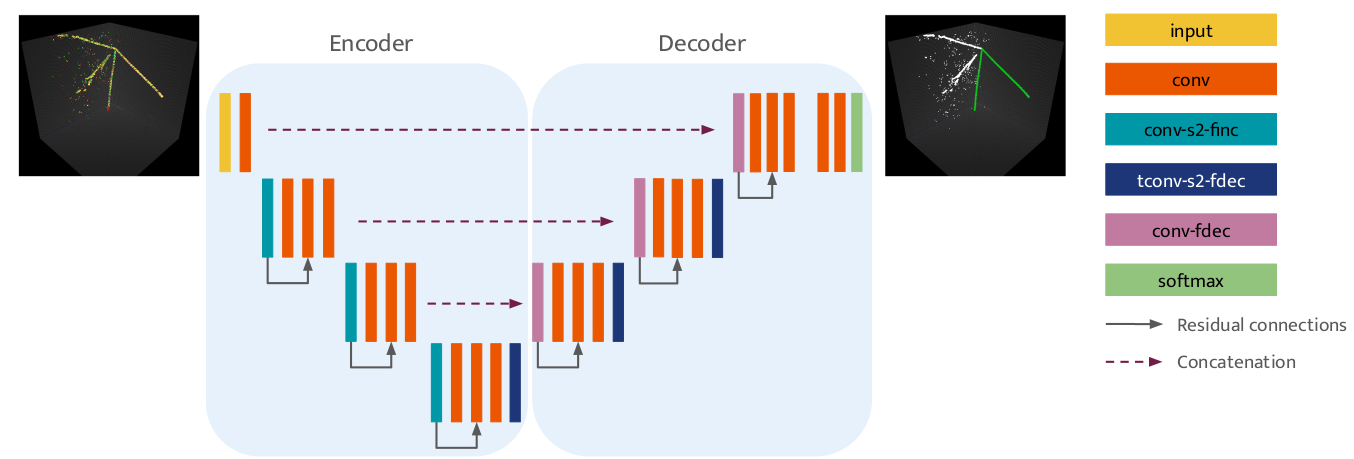
\includegraphics[width=120mm]{figures/uresnet.png}
  \caption{UResNet Architecture \cite{Drielsma_2024}}
  \label{uresnet}
\end{figure}

The semantic segmentation reconstruction is supposed to take the raw voxels and classify them into one of 5 or 6 categories based on whether ghost points are included in the dataset.

\begin{itemize}
\item Electromagnetic showers (e.g. electrons, photons = gammas)

\item Track-like particles (e.g. muons, protons, pions)

\item Delta rays (electrons knocked off from hard scattering)

\item Michel electrons (coming from muon decay)

\item Low energy depositions

\item Ghost points (if enabled) (Ambigous points from wire plane detectors)

\end{itemize}

Since the $2 \times 2$ has a pixellated readout plane, we don't have to worry about ghost points in this case.

\begin{figure}[H]
  % OWN
  \centering
  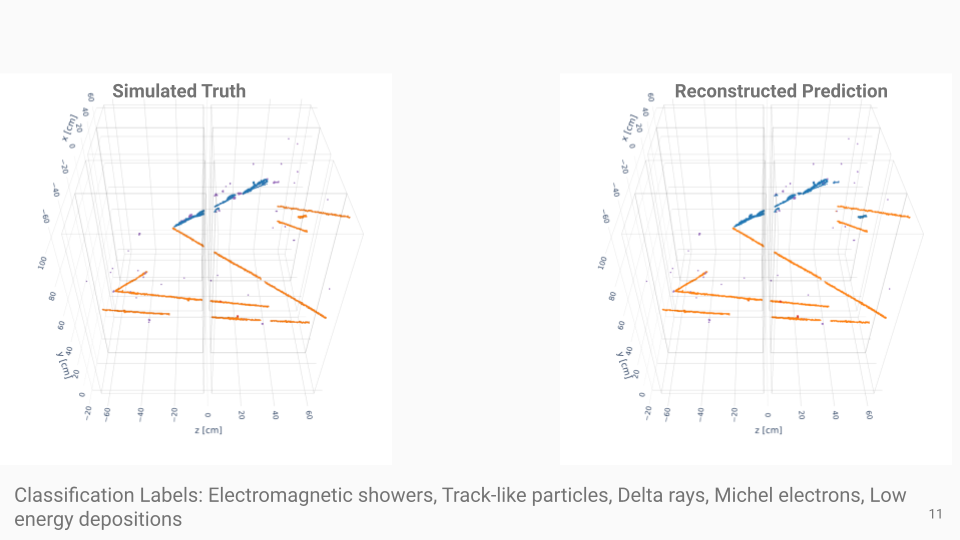
\includegraphics[width=120mm]{figures/semanticEvent.png}
  \caption{Semantic Segmentation Event display comparing monte carlo truth and reconstructed prediction}
  \label{semanticEvent}
\end{figure}

The other part of this step is the point proposal network (PPN).
This is just 3 layers attached to the UResNet model.
The job of the PPN is to pick out points of interest; namely the start of a shower, the start of a track and the end of a track \cite{Tilley_2021}.

The performance of this stage can be seen in figure \ref{semanticPerformance}.

\begin{figure}[H]
  % OWN
  \centering
  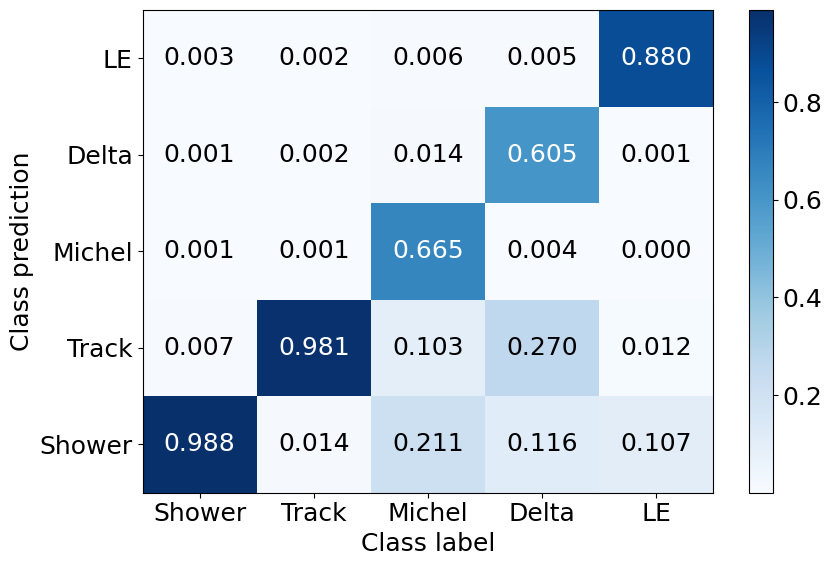
\includegraphics[width=120mm]{figures/semanticPerformance.png}
  \caption{Confusion Matrix showing performance of semantic segmentation}
  \label{semanticPerformance}
\end{figure}

Figure \ref{semanticPerformance}  is a confusion matrix. It has numbers that indicate how often the model is getting the right answers. The rows are predictions while the columns are the label from the simulation.
Basically, for every event, the network runs  and makes a prediction.
This prediction is then compared to the simulated truth.
Once all the events are run through, the percentages are calculated and the numbers put in the appropriate positions in the matrix.
The matrix shows that the model performs well at identifying tracks and showers but is still having  some difficulty with low energy depositions because it is harder to identify when it is a low energy deposition and when it should be part of something else.



The full SPINE pipeline was trained on a Set of 400k (train) + 100k (validation) 2x2 simulated images.
Isotropic particle bombs ($\nu$-like)overlayed with isotropic particles (rock-like)
So the performance numbers reflect this training environment.






